
% Subtypes analysis
\subsection{Differential Expression Analysis} \label{s:N_I:sel_tfs_subtypes}

% Metadata exploration
To understand better the biology of the small basal group, the metadata from TCGA \citet{Robertson2017-mg} was used. Several metadata features were explored: level of smoking (cigarettes per day), race, metastasis, relation to noninvasive bladder cancer, and histology grade. \Cref{fig:ap:sel_tfs_tcga_metadata} from Appendix displays this information in the form of multiple histograms, where the x-axes represent the subtypes derived in this section and the y-axes the count of the metadata features. From the figure, there is no immediate characteristic for the small basal group, neither with the Squamous pathology nor with the metastatic status, but most of the patients were smokers. It is worth pointing out that LumInf, Mes-like, and large luminal groups are generally characterised by non-squamous tumours. From Appendix \Cref{fig:ap:sel_tfs_tcga_meta_mut} shows that there is no immediate relationship with the mutations selected in the TCGA supplementary material, while \cref{fig:ap:sel_tfs_tcga_meta_apobec} (appendix) shows no relationship with the \textit{APOBEC} mutation.

% Pi plot for Small Ba/Sq
\begin{figure}[!htb]   
\centering
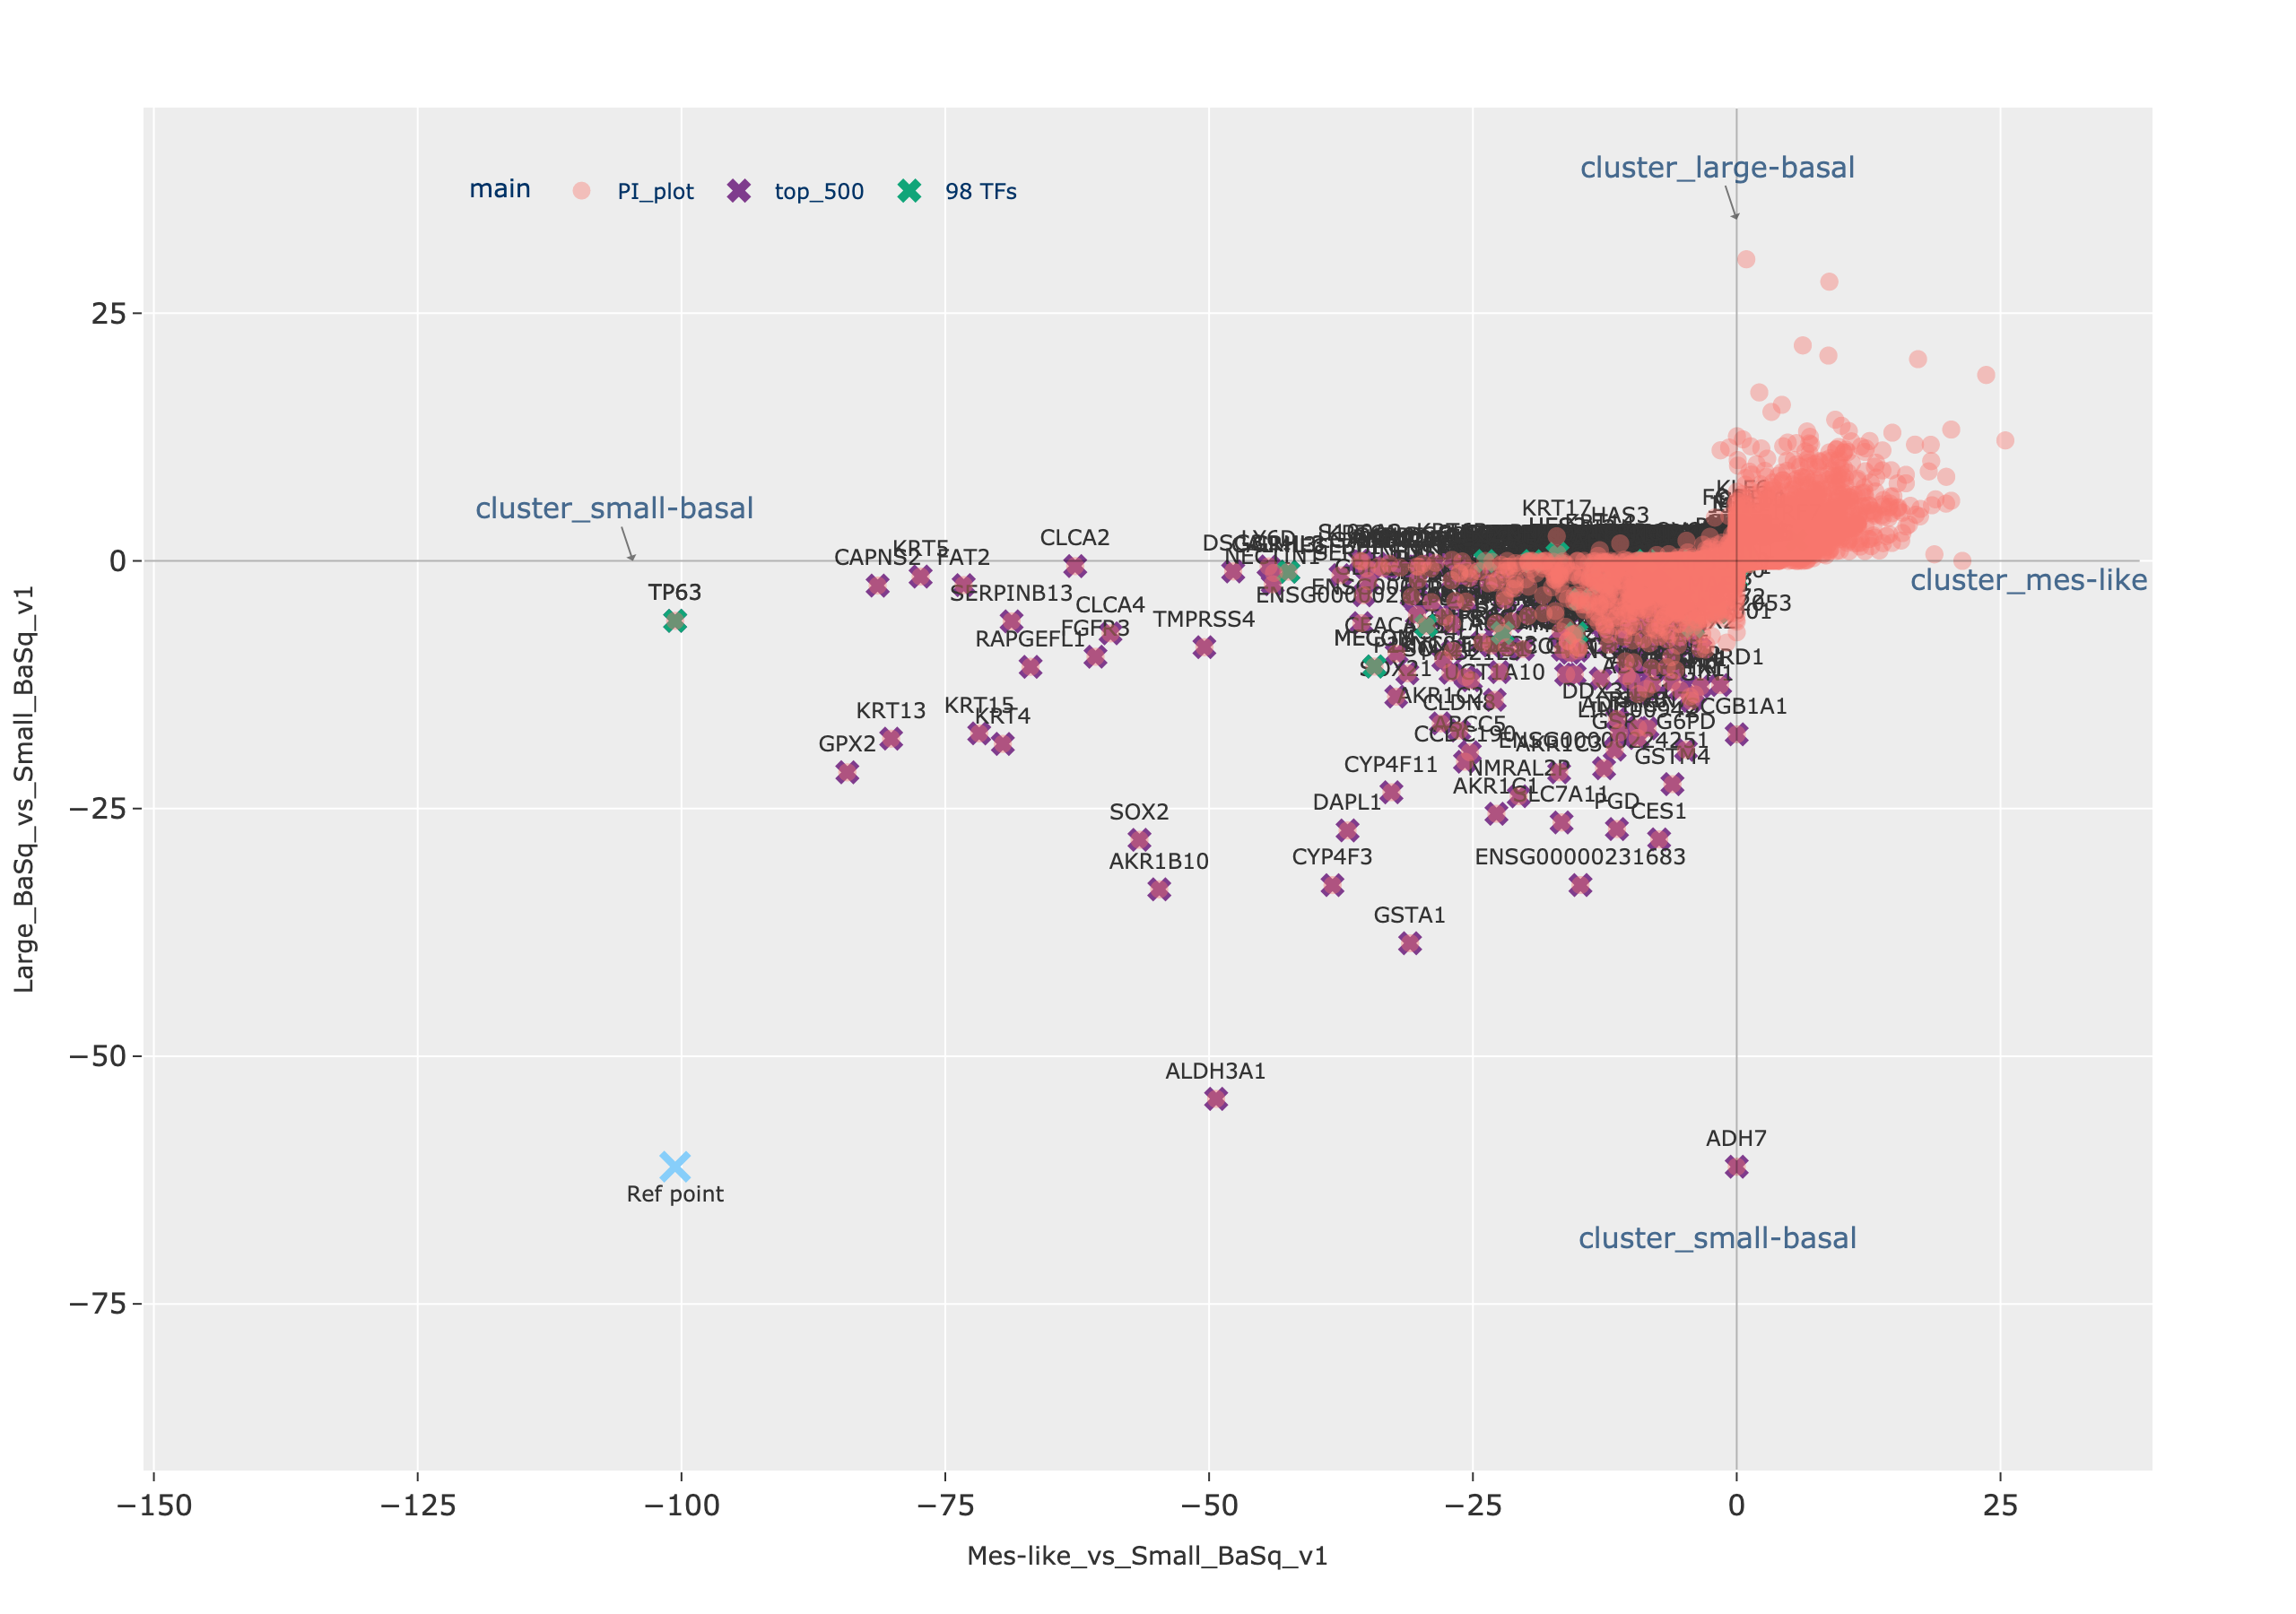
\includegraphics[width=1.0\textwidth,height=1.0\textheight,keepaspectratio]{Sections/Network_I/Resources/selective_pruning/pi_gsea/pi_smallBasal.png}
  \caption{Pi plot showing the Small Basal vs Large Basal on the X-axis, and Small-Basal vs Mes-like Y-axis. This plot highlights the genes that are high and significantly expressed in the Small Basal subtype. }
\label{fig:N_I:pi_smallBasal_comp}
\end{figure}

% pi plot
Differentially expressed analysis (DEA) was performed between the MIBC groups derived from the gene expression of the 98 TFs. The analysis enables to compare cancer subtypes beyond the transcription factors, and to find the genes that are significantly expressed to each subtype. For every MIBC group, a pi scatter plot is used as in \cref{fig:N_I:pi_smallBasal_comp}, where there is a quadrant (here - III) that holds the genes specific to that subtype with respect with the compared groups. In \cref{fig:N_I:pi_smallBasal_comp} the small basal (5 from \cref{fig:N_I:sel_tfs_cs_analysis}) is compared against the large basal, on the x-axis, in order to determine the properties over the other basal. The pi-values on the y-axis are the result from small-basal vs mes-like as it was observed that the mes-like group is different from both the luminal\footnote{The purpose of the pi plot was to highlight the specific genes to the small-basal. However, one may think that a more direct comparison of the small-basal with the luminal groups could have been chosen, instead of mes-like DEA. The other pi-plots comparison (like the plots for LumInf,  large luminal \cref{fig:ap:pi_other_values_I,fig:ap:pi_other_values_II} - in Appendix) cover the 'basal' vs 'luminal' comparison. }. The light-blue marker in quadrant III represents the referential point to which the genes are 'the most' enriched in the small-basal, and the closest 500 genes to the referential point are coloured in purple. 


% Introduce the GSEA
The distance to the referential marker is computed for each point in the scatter plot \cref{fig:N_I:pi_smallBasal_comp} and then ranked in descending order. This means that all the points in the pi-plot are ranked by how much these are differentially and significantly are expressed in the small basal group. It also allows to run the pre-rank method for Gene Set Enrichment Analysis (GSEA) using the \textit{GSEAPY} library \citet{Fang2023-ec}. The pre-rank GSEA was configured to 1000 permutations (lowering the chance of misidentifying pathways) and the False Discovery Rate (FDR) of the q-value was kept at 0.05. The same process was repeated for the other subtypes based on their corresponding pi-plots\footnote{The pi-plot figures were also used to verify the results from GSEA. The genes found in the top pathways were plotted back on the plot to check if these are in the quadrant specific to the subtype studied.}; see \cref{s:ap:sel_prun_pi}.

% Why the top terms are kept
Taking a step back, the input data for GSEA for each subtype is taking the same (large) list of genes but it is ranked differently, giving more importance to the genes specific to the studied subtypes. The GSEA results will then shared a large number of found pathways at each run. To address this, the ten terms with the highest normalised enrichment score (NES) were kept for each MIBC subtype GSEA run. Having a restricted subset of term allows to find the exclusive pathways for a subgroup. Reactome 2023 v2 was used as the database to search for pathways in this section as it contains the up-to-date canonical pathways, it is medium size (1692 gene sets) as well the names are easier to interpret The output from the GSEA can be seen in which can be seen in the tables \cref{tab:N_I:gsea_basal_reactome,tab:N_I:gsea_luminal_reactome}.

% GSEA basal table (reactome)
\begin{table}[H]
  \centering
  \scriptsize
  \begin{tabularx}{\textwidth}{>{\hsize=1.7\hsize}X|>{\hsize=0.4\hsize}X|>{\hsize=0.4\hsize}X|>{\hsize=0.6\hsize}X|>{\hsize=0.4\hsize}X|>{\hsize=0.15\hsize}X}
    \toprule
    \textbf{Term} & \textbf{NES} & \textbf{FDR q-val} & \textbf{\# lead} & \textbf{\# matched} & \textbf{ratio} \\
    \midrule
    \multicolumn{6}{c}{\textbf{smallBasal}} \\
    \midrule
    NFE2L2 REGULATING ANTI OXIDANT DETOXIFICATION ENZYMES & 2.486 & 0 & 13 & 13 & 1 \\
    \midrule
    RND1 GTPASE CYCLE & 2.158 & 0 & 31 & 23 & 0.742 \\
    \midrule
    REGULATION OF RUNX1 EXPRESSION AND ACTIVITY & 2.114 & 0 & 11 & 8 & 0.727 \\
    \midrule
    SIGNALING BY PDGFR IN DISEASE & 2.101 & 0 & 13 & 9 & 0.692 \\
    \midrule
    RORA ACTIVATES GENE EXPRESSION & 2.082 & 0 & 15 & 13 & 0.867 \\
    \midrule
    GLUTATHIONE CONJUGATION & 2.063 & 0 & 20 & 17 & 0.85 \\
    \midrule
    ACYL CHAIN REMODELLING OF PC & 2.061 & 0 & 12 & 12 & 1 \\
    \midrule
    DOWNREGULATION OF ERBB2 SIGNALING & 2.034 & 0 & 14 & 14 & 1 \\
    \midrule
    SIGNALING BY ERBB2 & 2.034 & 0 & 25 & 25 & 1 \\
    \midrule
    ACTIVATION OF GENE EXPRESSION BY SREBF SREBP & 2.021 & 0 & 33 & 25 & 0.758 \\
    \midrule
    \multicolumn{6}{c}{\textbf{largeBasal}} \\
    \midrule
    INTERLEUKIN 10 SIGNALING & 2.561 & 0 & 37 & 37 & 1 \\
    \midrule
    PARASITE INFECTION & 2.545 & 0 & 89 & 84 & 0.944 \\
    \midrule
    INTERFERON ALPHA BETA SIGNALING & 2.489 & 0 & 46 & 46 & 1 \\
    \midrule
    SIGNALING BY THE B CELL RECEPTOR BCR & 2.482 & 0 & 137 & 111 & 0.81 \\
    \midrule
    FCGAMMA RECEPTOR FCGR DEPENDENT PHAGOCYTOSIS & 2.479 & 0 & 102 & 97 & 0.951 \\   
    \bottomrule
  \end{tabularx}
  \caption{Normalised Enrichment Score (NES), False Discovery Rate (FDR) q-val, and lead gene statistics for the two basal groups. The lead genes from a pathway are selected by GSEAPY based on when the NES reached its peak.}
  \label{tab:N_I:gsea_basal_reactome}
\end{table}

The GSEA output tables contain the Normalised enrichment score (NES), the False-Discovery Rate (FDR) of the q-value and lead genes statistics. A gene or a subset of genes are considered lead genes the ones where the enrichment score peaked. The 5000 closest genes to the referential point for each subtype (see \cref{fig:N_I:pi_smallBasal_comp}) are then intersected wit the lead genes, given the '\# matched' and 'ratio' columns in the tables \cref{tab:N_I:gsea_basal_reactome,tab:N_I:gsea_luminal_reactome} and the GSEA results for hallmarks and Onco Signature database from Appendix \cref{ap:tab:gsea_hallmark,ap:tab:gsea_oncosig}.

\begin{figure}[!htb]   
\centering
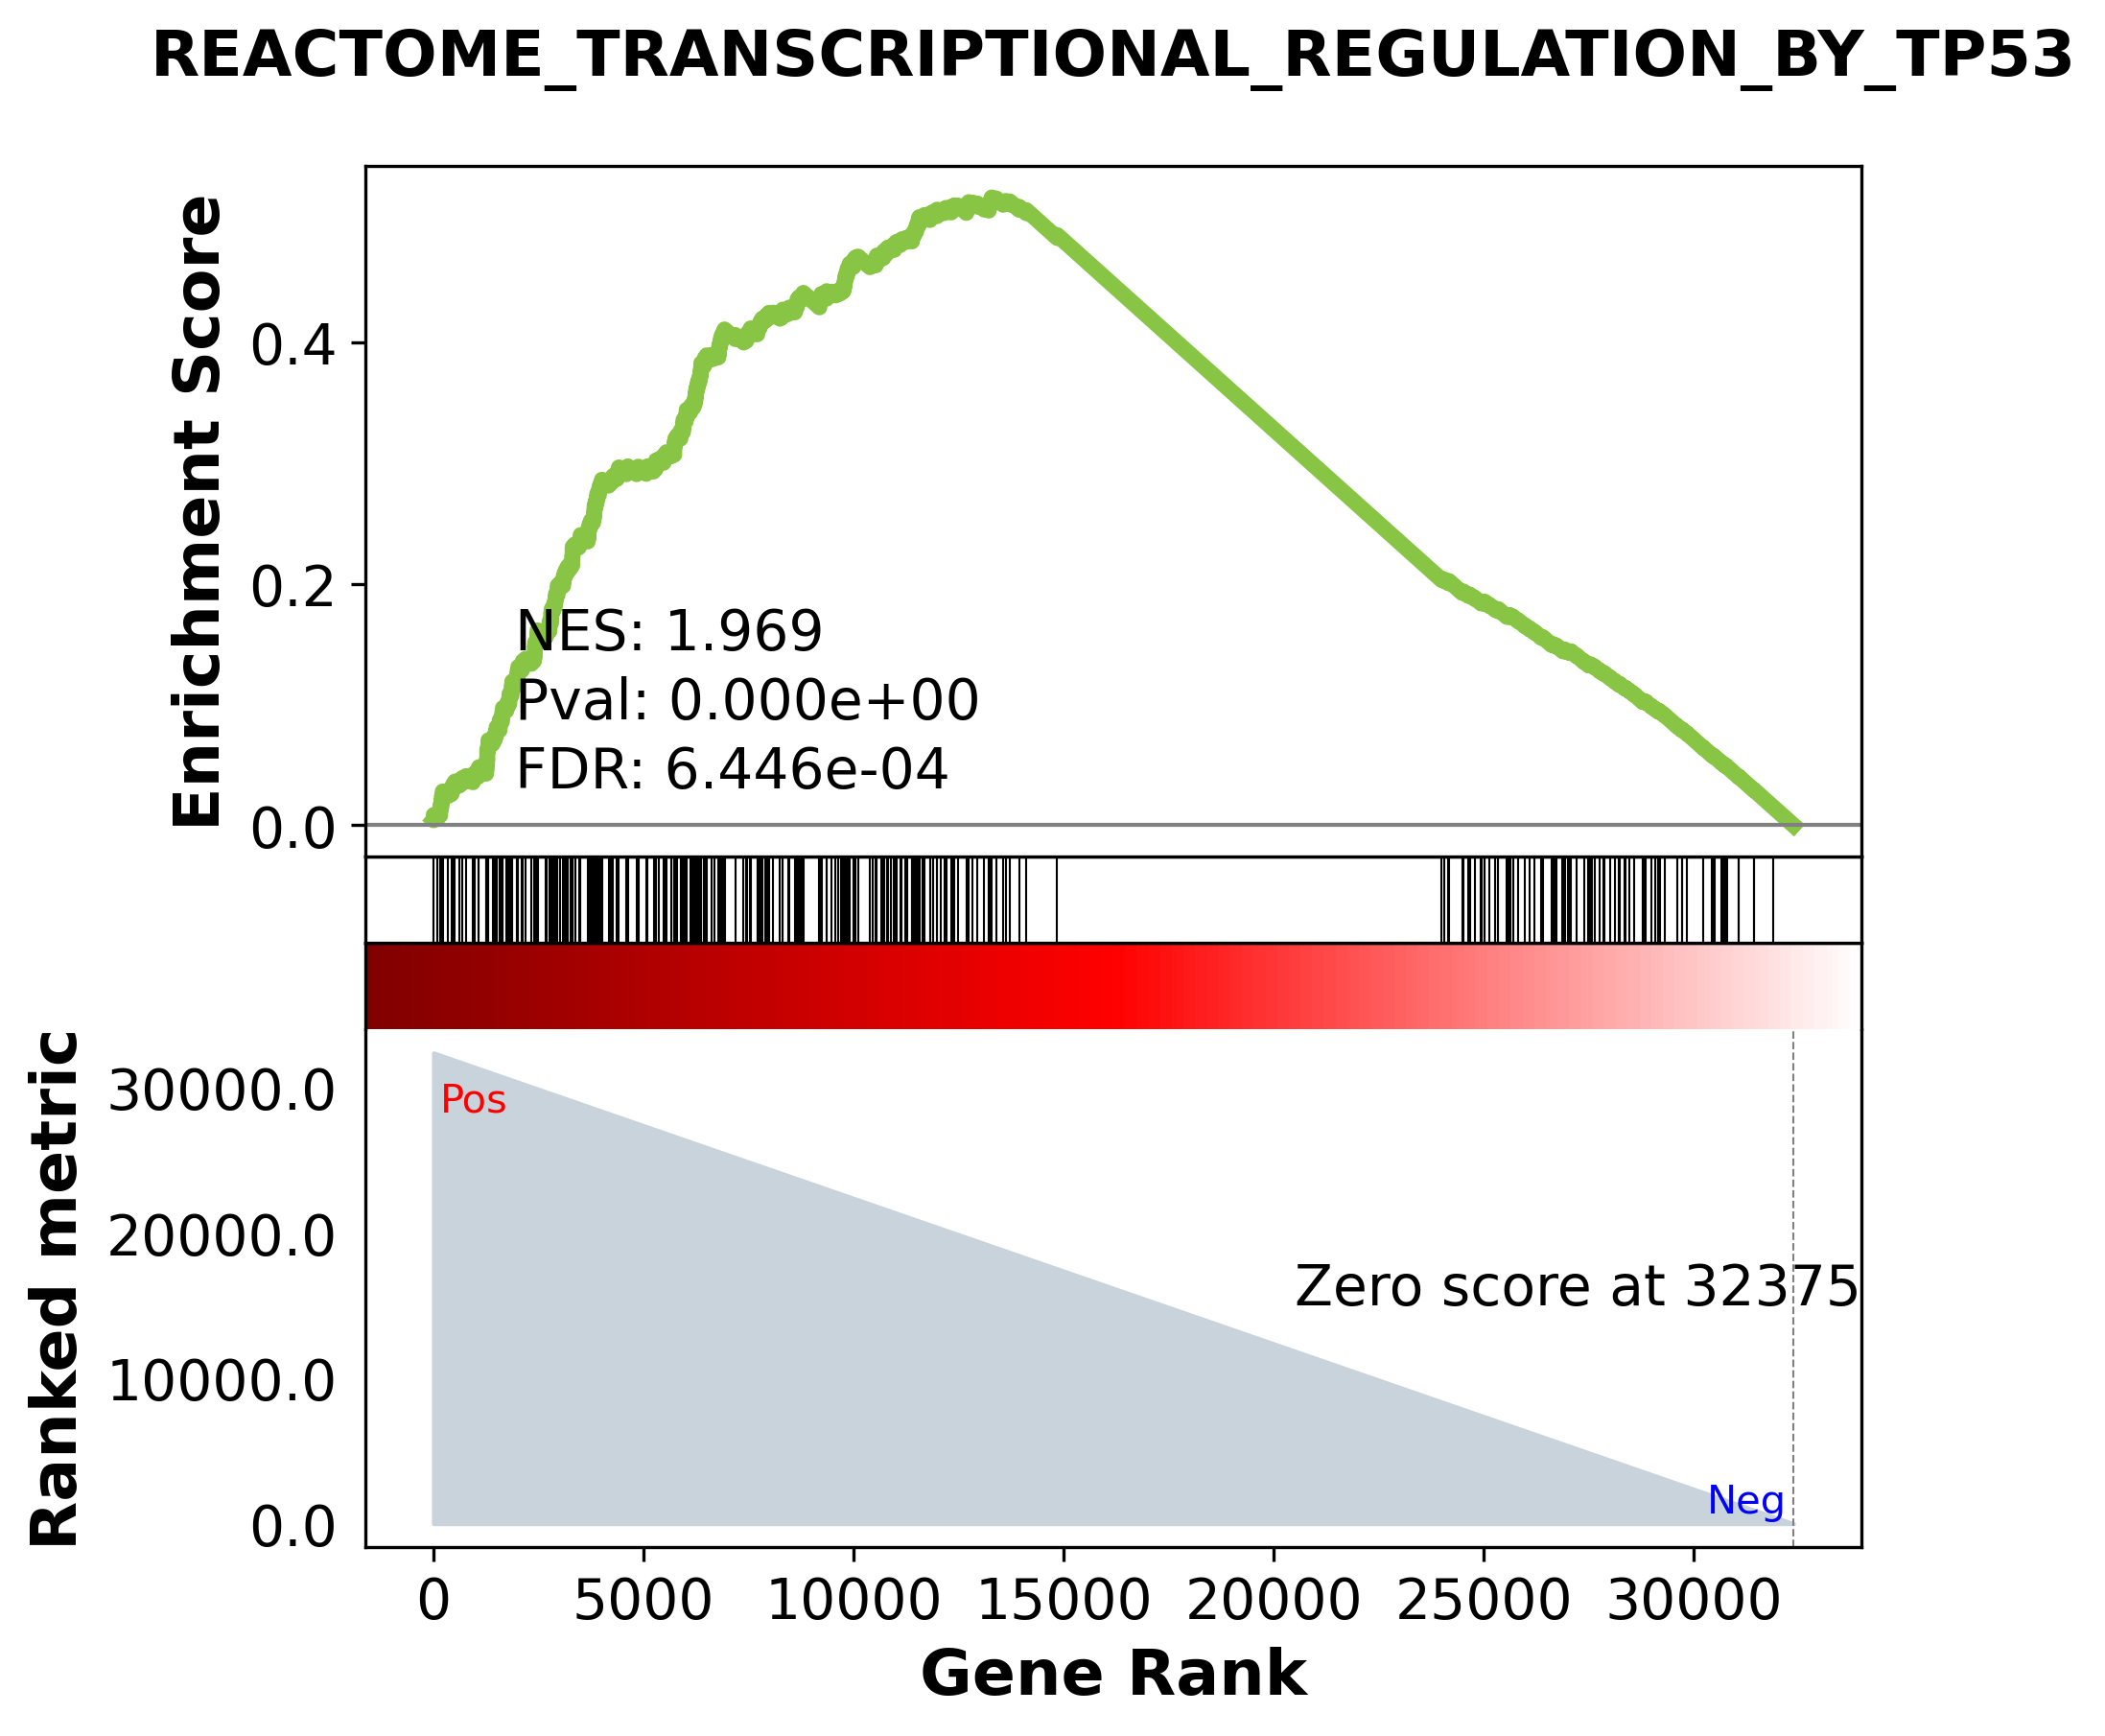
\includegraphics[width=0.7\textwidth,height=0.7\textheight,keepaspectratio]{Sections/Network_I/Resources/selective_pruning/gsea/REACTOME_TRANSCRIPTIONAL_REGULATION_BY_TP53.png}
  \caption{GSEA plot for the p53 pathway found in the smaller basal group. While there is a strong enrichment of this pathway is not unique to this group.}
\label{fig:N_I:gsea_p53_smallBasal}
\end{figure}

% Small basal commenting
The first part of the table \cref{tab:N_I:gsea_basal_reactome} contains the pathways found for the small basal group which are most involved in the cell functioning. It is striking that in most of the pathways found the lead genes are matched by the 5000 genes closest to the referential point. This denotes that from the 5000 genes there are many which play an important role in multiple pathways. Disruption to the cell cycle may also explain the poor survival prognosis. As seen in the GSEA plot from \cref{fig:ap:gsea_smallBasal}, the enrichment score is high but not many genes are hit in the high ranked genes (i.e. top 5000) and the most hit pathways is "NFE2L2 regulating anti oxidant detoxification enzymes". In the previous analysis done in this section suggested that \textit{TP53} is a marker for the smaller group. There is a 
strong signal of the \textit{p53} pathway as seen in \cref{fig:N_I:gsea_p53_smallBasal} but it is not unique to the smaller group.

% large basal commenting
In the second part of the \cref{tab:N_I:gsea_basal_reactome}, the pathways for the larger basal group are presented, which are mostly related to the immune response of the tissue. Especially the high match of the interferon pathways, which is expected as this groups contains the subtypes which were classified in the previous section \cref{s:clustering_analysis} as Medium IFNG and High IFNG. There was no unique signature found for Mes-like subgroup as the subtype shares pathways with the basal groups (interferon alpha, gamma pathways) as seen in the GSEA outputs from appendix \cref{fig:ap:gsea_largeBasal,fig:ap:gsea_mesLike}.

The table \cref{tab:N_I:gsea_luminal_reactome} contains the pathways found for the larger and infiltrated luminal subtypes. The pathway for latter mostly contains immunoglobulin related genes (e.g. \textit{IGV1-17}) denoting the infiltration of the immune cells in the bladder cancer samples. The pathways found for the large luminal are general and the lead genes have a low match ratio with the most 5000 most representative genes. This suggests that there is a less of a clear signal for a pathway to be enriched which might be explained by the size of the luminal group. 

% GSEA luminal table (reactome)
\begin{table}[!t]
  \centering
  \scriptsize
  \begin{tabularx}{\textwidth}{>{\hsize=1.7\hsize}X|>{\hsize=0.4\hsize}X|>{\hsize=0.4\hsize}X|>{\hsize=0.6\hsize}X|>{\hsize=0.4\hsize}X|>{\hsize=0.15\hsize}X}
    \toprule
    \textbf{Term} & \textbf{NES} & \textbf{FDR q-val} & \textbf{\# lead} & \textbf{\# matched} & \textbf{ratio} \\
    \midrule
    \multicolumn{6}{c}{\textbf{lumInf}} \\
    \midrule
    SCAVENGING OF HEME FROM PLASMA & 2.396 & 0 & 54 & 47 & 0.87 \\
    \midrule
    \multicolumn{6}{c}{\textbf{largeLuminal}} \\
    \midrule
    PARACETAMOL ADME & 2.016 & 0.003 & 15 & 15 & 1 \\
    \midrule
    EUKARYOTIC TRANSLATION ELONGATION & 1.864 & 0.029 & 73 & 5 & 0.068 \\
    \midrule
    SELENOAMINO ACID METABOLISM & 1.86 & 0.02 & 80 & 4 & 0.05 \\
    \midrule
    NONSENSE MEDIATED DECAY NMD & 1.832 & 0.025 & 81 & 8 & 0.099 \\
    \midrule
    SRP DEPENDENT COTRANSLATIONAL PROTEIN TARGETING TO MEMBRANE & 1.828 & 0.022 & 80 & 6 & 0.075 \\
    \midrule
    FORMATION OF WDR5 CONTAINING HISTONE MODIFYING COMPLEXES & 1.827 & 0.018 & 25 & 7 & 0.28 \\
    \midrule
    RESPONSE OF EIF2AK4 GCN2 TO AMINO ACID DEFICIENCY & 1.809 & 0.019 & 73 & 4 & 0.055 \\
    \midrule
    MITOCHONDRIAL FATTY ACID BETA OXIDATION & 1.789 & 0.023 & 28 & 18 & 0.643 \\
    \midrule
    BRANCHED CHAIN AMINO ACID CATABOLISM & 1.777 & 0.024 & 9 & 9 & 1 \\
    \midrule
    EUKARYOTIC TRANSLATION INITIATION & 1.77 & 0.025 & 76 & 5 & 0.066 \\
    \bottomrule
  \end{tabularx}
  \caption{Normalised Enrichment Score (NES), False Discovery Rate (FDR) q-val, and lead gene statistics for the large, infiltrated and mes-like group. The lead genes from a pathway are selected by GSEAPY based on when the NES reached its peak.}
  \label{tab:N_I:gsea_luminal_reactome}
\end{table}

GSEA was also applied to the hallmark gene set (50 pathways) and the oncogenic signature (189 gene sets), results that can be seen in Appendix \cref{ap:tab:gsea_hallmark,ap:tab:gsea_oncosig}. The GSEA outputs are harder to interpret especially the Onco Signature sets, but it can be observed that most of the unique pathways are found in both small basal and large luminal groups. Considering that the small basal group is considerably smaller than the large luminal, it suggests that the subtype should be study more.


% What are these 10 top genes
Returning to the small group and the pi scatter plot from \cref{fig:N_I:pi_smallBasal_comp},
seven out of the ten genes closest to the referential point were found to have biological significance in bladder cancer biology: \textit{GPX2, KRT13, ALDH3A1, KRT15, KRT4, AKR1B10, SOX2, TP63, RAPGEFL1, CAPNS2}. \textit{GPX2} is involved in squamous differentiation \citet{Naiki2018-fp}. Higher expression of \textit{KRT13} is associated with better response to chemotherapy and immunotherapy \citet{Yu2023-db}. The methylation of \textit{ALDH3A1}, along with \textit{HOXA9} and \textit{ISL1}, has been studied in non-muscle invasive bladder cancer and found to be a predictor of disease recurrence \citet{McLean2023-qk}. Additionally, higher expression of \textit{ALDH3A1} in bladder cancer is associated with higher tumour grade and has been studied in cancer stem cells \citet{Kim2013-th}. \textit{KRT4} is a basal keratin marker \citet{Marzouka2018-ge}. Both \textit{AKR1B10} and \textit{SOX2} are associated with cell and cancer aggressiveness \citet{Huang2021-bn, Chiu2020-xh}, while \textit{TP63} is a known squamous marker \citet{Robertson2017-mg}. This evidence supports the poor survival prognosis of the smaller group and indicates that this group warrants further study.